\chapter{Fuerzas, espacio de fases y leyes de conservación}

\lectureoverview{Una ley del movimiento debe hacer algo más que relacionar magnitudes físicas conocidas. Debe especificar el estado de un sistema, llevarlo de un instante al siguiente y revelar qué distinciones y magnitudes se mantienen durante el movimiento. Llegaremos a la mecánica newtoniana poniendo primero a prueba una ley de fuerza plausible pero errónea; después ampliaremos el estado, desde la posición hasta el espacio de fases, y, por último, deduciremos la conservación del momento y de la energía.}

\section{Una ley errónea, pero útil}

El movimiento cotidiano está dominado por el rozamiento. Empujamos un objeto pesado por el suelo y se mueve; dejamos de empujarlo y pronto se detiene. Por lo general, un empuje mayor produce una velocidad mayor, mientras que un objeto más pesado requiere un empuje más intenso. En un mundo así, es natural suponer que la fuerza produce la propia velocidad. Esta era la intuición básica de la descripción aristotélica del movimiento.

El patinaje sobre hielo aporta la experiencia que falta. Un patinador necesita ejercer una fuerza para arrancar, detenerse o cambiar de dirección, pero no para seguir deslizándose una vez que está en movimiento. Si Aristóteles hubiera trabajado sobre hielo casi sin rozamiento, en vez de sobre suelo ordinario, habría sido mucho más difícil pasar por alto el defecto de la intuición fuerza--velocidad.

Para dejar claro qué falla en esa intuición, démosle una formulación moderna precisa. Escribimos la ecuación deliberadamente incorrecta

\begin{equation}
  \mathbf F=m\mathbf v.
  \label{eq:aristotle-vector-law}
\end{equation}

Esta no es la ley de Newton y no debe memorizarse como física. Su utilidad es diagnóstica: una vez que una regla verbal se expresa mediante una ecuación, podemos preguntar si predice el movimiento y si conserva suficiente información para reconstruir el pasado. La breve discusión en clase sobre la palabra griega para fuerza remite a \emph{dynamis}, raíz que también se reconoce en palabras como dinamo y dinámica; pero la terminología es secundaria frente a la prueba de la propia ley.

\begin{figure}[htbp]\centering
  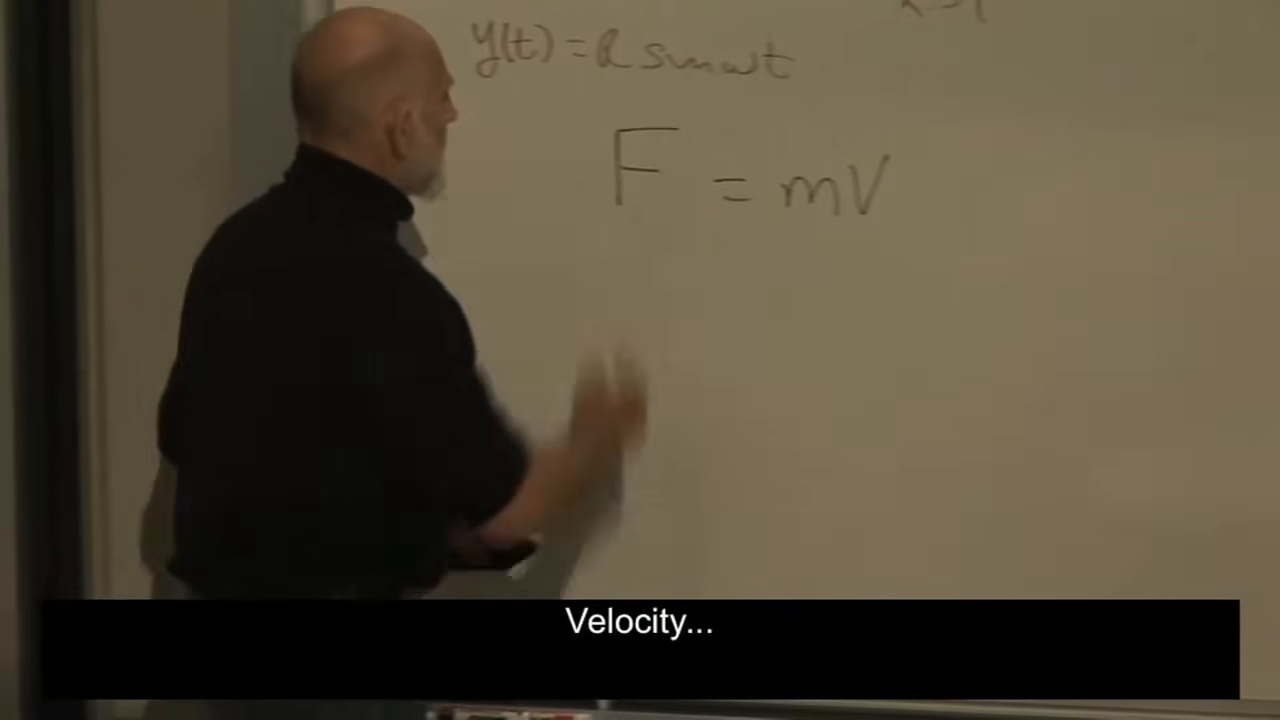
\includegraphics[width=0.82\textwidth]{lecture_02_figure_02.png}\caption{La ley fuerza--velocidad, deliberadamente errónea, que se usa para poner a prueba la predictibilidad y la reversibilidad.}\lectureframe{00:04:51}\end{figure}

Restringimos el movimiento a una sola coordenada espacial. Como \(v=\dot x\), la ley es

\begin{equation}
  F(t)=m\dot x(t).
  \label{eq:aristotle-1d}
\end{equation}

Dividamos ahora el tiempo en intervalos cortos de longitud \(\delta\). Durante un intervalo,

\begin{equation}
  \dot x(t)\simeq
  \frac{x(t+\delta)-x(t)}{\delta}.
  \label{eq:first-difference}
\end{equation}

Al sustituir en la ecuación~\eqref{eq:aristotle-1d}, obtenemos

\begin{equation}
  x(t+\delta)
  =x(t)+\frac{\delta}{m}F(t).
  \label{eq:aristotle-update}
\end{equation}

Esto tiene la forma de una regla de actualización genuina. Si conocemos la posición actual y la fuerza, se obtiene la posición en el siguiente instante estroboscópico. Sin embargo, cuando la fuerza se anula, la regla de Aristóteles da \(\dot x=0\): el objeto debe permanecer en reposo. Desde el principio, queda excluido el movimiento sin una fuerza que lo sostenga.

\begin{figure}[htbp]\centering
  \includegraphics[width=0.84\textwidth]{lecture_02_figure_07.png}\caption{La actualización discreta de Aristóteles con una fuerza restauradora. En cada paso, el desplazamiento se multiplica por un factor ligeramente menor que uno.}\lectureframe{00:10:15}\end{figure}

\subsection{Un resorte en la mecánica de Aristóteles}

Consideremos una partícula unida a un resorte, cuyo equilibrio se encuentra en \(x=0\). Un desplazamiento produce la fuerza restauradora

\begin{equation}
  F(x)=-kx,
  \qquad k>0.
  \label{eq:hooke-law}
\end{equation}

Al introducir esta fuerza en la ecuación~\eqref{eq:aristotle-update}, se obtiene

\begin{equation}
  x(t+\delta)
  =\left(1-\frac{k\delta}{m}\right)x(t).
  \label{eq:aristotle-spring-update}
\end{equation}

Para valores suficientemente pequeños de \(\delta\), el factor entre paréntesis es apenas menor que uno. Por tanto, cada actualización reduce el desplazamiento en la misma proporción:

\begin{equation}
  x_n=\left(1-\frac{k\delta}{m}\right)^n x_0.
  \label{eq:aristotle-geometric-decay}
\end{equation}

La ecuación continua y su solución son

\begin{align}
  m\dot x&=-kx,
  \label{eq:aristotle-spring-continuous}\\
  x(t)&=x(0)e^{-kt/m}.
  \label{eq:aristotle-spring-solution}
\end{align}

El resorte no oscila. Si se suelta desde cualquier desplazamiento, se aproxima exponencialmente al origen y avanza cada vez más despacio a medida que llega a él.

\begin{figure}[htbp]\centering
  \includegraphics[width=0.84\textwidth]{lecture_02_figure_08.png}\caption{La solución exponencial de la ecuación aristotélica del resorte. El desplazamiento decae en vez de oscilar.}\lectureframe{00:12:02}\end{figure}

El futuro es fácil de predecir: cualquier desplazamiento inicial se aproxima a la misma configuración de reposo. El pasado es otra cuestión. Supongamos que observamos la partícula muy cerca del origen, con una precisión finita. Podría haber partido de cualquiera de muchos desplazamientos distintos, porque, con el tiempo, todos sus restos exponencialmente pequeños acaban dentro de la misma tolerancia de medida. Con precisión matemática perfecta, la ecuación~\eqref{eq:aristotle-spring-solution} puede recorrerse hacia atrás, pero las distinciones prácticas entre las historias se borran de manera continua. Por ello, desde el punto de vista de la dinámica fundamental reversible, la ley resulta sospechosa.

Esto no significa que Aristóteles fuera irracional. El movimiento dominado por el rozamiento que describió es, en efecto, disipativo. El error consistió en elevar ese comportamiento efectivo a la categoría de ley fundamental. El rozamiento es, a su vez, una fuerza que surge de interacciones microscópicas complejas. Cuando una mano empuja un objeto a velocidad aproximadamente constante, la fuerza aplicada equilibra el rozamiento; no está creando la velocidad como tal.

\section{La ley de Newton y su significado físico}

La corrección newtoniana consiste en que la fuerza cambia el movimiento:

\begin{equation}
  \mathbf F=m\mathbf a=m\ddot{\mathbf x}.
  \label{eq:newton-second-law}
\end{equation}

Antes de tratar esto como una ecuación de evolución, hay que desenredar dos aparentes circularidades. La primera se refiere a los sistemas de referencia. A menudo se dice que las leyes de Newton se cumplen en sistemas inerciales y que un sistema inercial es aquel en el que se cumplen las leyes de Newton. La afirmación física no es esa definición circular. Es la afirmación empírica de que \emph{existen} sistemas, descritos mediante reglas y relojes adecuados, en los que las leyes de Newton adoptan su forma sencilla. Los sistemas que aceleran o giran con respecto a ellos requieren fuerzas aparentes adicionales. Más adelante se puede determinar cómo se transforman las ecuaciones en esos otros sistemas.

La segunda circularidad se refiere a la fuerza y la masa. Si la fuerza se define como masa por aceleración y la masa como fuerza dividida por aceleración, la ecuación parece vacía. Un experimento operacional separa las definiciones de la ley. Compare un objeto con un kilogramo patrón equilibrándolos y, luego, una el objeto a una balanza de resorte en un espacio sin fuerzas de otro tipo. Defina una unidad de fuerza mediante una pequeña extensión fija del resorte. Dos resortes idénticos, cada uno estirado esa misma cantidad, proporcionan dos unidades de fuerza y producen el doble de aceleración. Es más seguro añadir un segundo resorte que estirar uno solo el doble, porque un resorte real acaba comportándose de manera no lineal o se rompe. Si se conserva un solo resorte y se unen dos masas iguales, la aceleración se reduce a la mitad; con tres masas iguales, se reduce a un tercio.

\begin{figure}[htbp]\centering
  \includegraphics[width=0.84\textwidth]{lecture_02_figure_09.png}\caption{Experimento mental con una balanza de resorte para definir unidades iguales de fuerza y comprobar que la aceleración es proporcional a la fuerza.}\lectureframe{00:22:45}\end{figure}

Estas comparaciones dan contenido empírico a

\begin{equation}
  a\propto F,
  \qquad
  a\propto\frac{1}{m},
  \qquad
  F=ma.
  \label{eq:force-mass-scaling}
\end{equation}

Usaremos la palabra \emph{partícula} para referirnos a cualquier objeto pequeño cuya estructura interna sea irrelevante, no solo a una partícula elemental.

\subsection{Por qué la posición no basta para definir un estado}

Ahora ponemos a prueba la ecuación de Newton con el mismo método estroboscópico. La diferencia finita centrada para la aceleración es

\begin{equation}
  \ddot x(t)\simeq
  \frac{x(t+\delta)-2x(t)+x(t-\delta)}{\delta^2}.
  \label{eq:second-difference}
\end{equation}

Así, la ecuación de Newton implica

\begin{equation}
  x(t+\delta)
  =2x(t)-x(t-\delta)+\frac{\delta^2}{m}F(t).
  \label{eq:newton-position-update}
\end{equation}

La posición siguiente no se puede obtener solo a partir de \(x(t)\). También necesitamos la posición anterior \(x(t-\delta)\) o, de manera equivalente, la velocidad en el instante actual. A primera vista, esto hace que la ecuación de Newton parezca menos predictiva que la de Aristóteles. La conclusión correcta es, en cambio, que la posición por sí sola era una descripción incompleta del estado. Conocer todo lo relevante en un instante significa conocer datos suficientes para determinar el movimiento posterior. Para una partícula newtoniana, esos datos son la posición y la velocidad.

\section{Momento y espacio de fases}

Introduzcamos el momento mediante

\begin{equation}
  \mathbf p=m\mathbf v=m\dot{\mathbf x}.
  \label{eq:momentum-definition}
\end{equation}

Se considera que la masa de un sistema newtoniano fijo es constante. Un objeto puede perder una pieza, como un bolígrafo puede perder el capuchón, pero entonces ha cambiado el objeto que se describe; el sistema cerrado elegido sigue teniendo masa total constante. Si \(m\) es constante, la segunda ley de Newton se convierte en

\begin{equation}
  \mathbf F=\dot{\mathbf p}.
  \label{eq:newton-momentum-form}
\end{equation}

\begin{figure}[htbp]\centering
  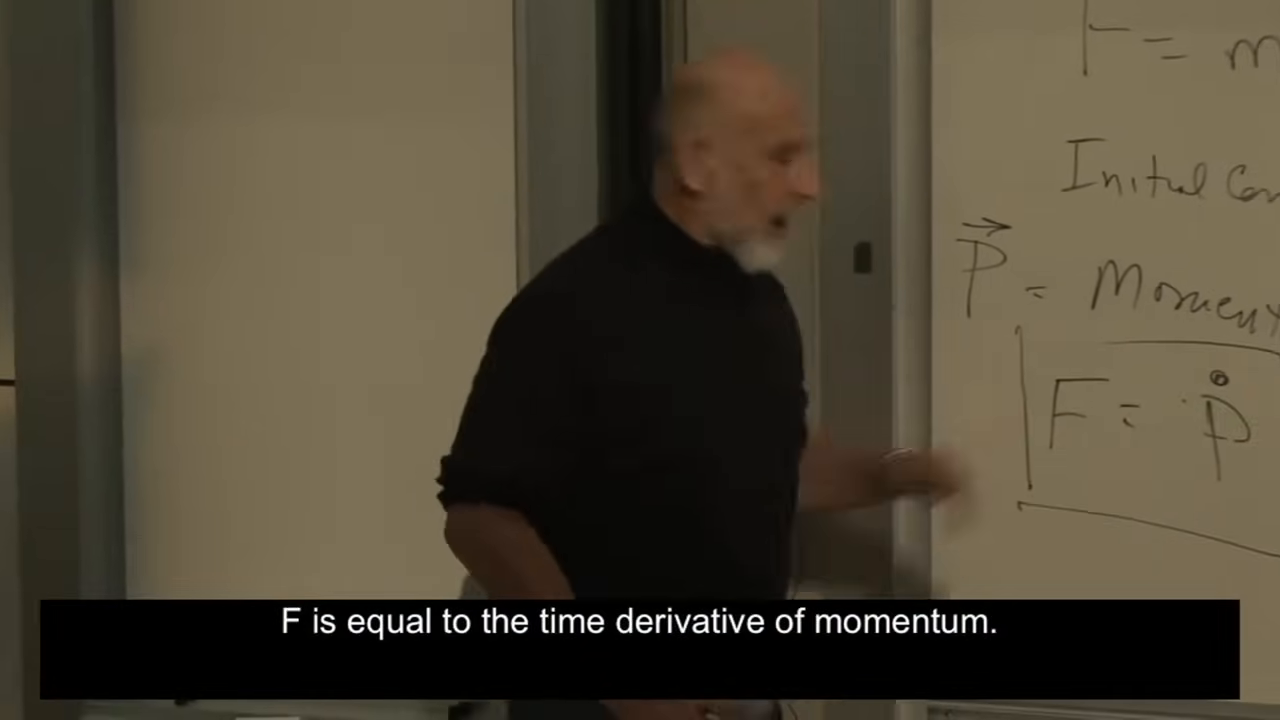
\includegraphics[width=0.82\textwidth]{lecture_02_figure_03.png}\caption{La ley de Newton expresada como derivada temporal del momento.}\lectureframe{00:32:35}\end{figure}

Para una coordenada, el movimiento newtoniano puede escribirse ahora como dos ecuaciones de primer orden para dos variables de estado independientes:

\begin{align}
  \dot p&=F(x,t),
  \label{eq:first-order-p}\\
  \dot x&=\frac{p}{m}.
  \label{eq:first-order-x}
\end{align}

Una ecuación indica cómo la fuerza cambia el momento; la otra, cómo el momento cambia la posición. Su forma discreta de primer orden es

\begin{align}
  p(t+\delta)&=p(t)+\delta F(x(t),t)+O(\delta^2),
  \label{eq:momentum-discrete}\\
  x(t+\delta)&=x(t)+\frac{\delta}{m}p(t)+O(\delta^2).
  \label{eq:position-discrete}
\end{align}

Dados \(x(t)\) y \(p(t)\), estas ecuaciones determinan el siguiente par, que pasa a ser la entrada para el paso posterior. La trayectoria se construye mediante actualizaciones sucesivas.

\begin{figure}[htbp]\centering
  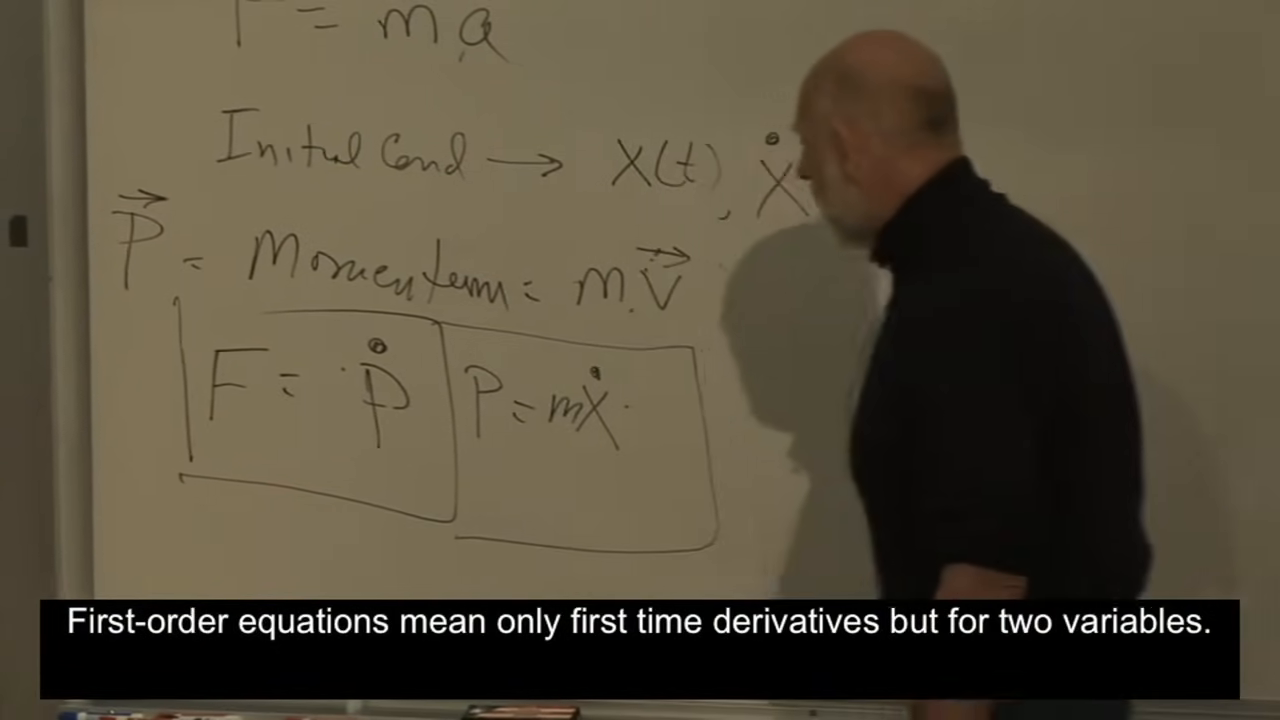
\includegraphics[width=0.84\textwidth]{lecture_02_figure_04.png}\caption{Las dos ecuaciones de primer orden y los datos iniciales correspondientes. La posición y el momento, en conjunto, especifican el estado.}\lectureframe{00:35:47}\end{figure}

El espacio de todos los pares \((x,p)\) se denomina \emph{espacio de fases}. Para una partícula que se mueve en tres dimensiones tiene seis coordenadas:

\begin{equation}
  (x,y,z,p_x,p_y,p_z).
  \label{eq:one-particle-phase-space}
\end{equation}

El espacio de fases es el espacio de las condiciones iniciales completas. El espacio de configuración registra solo las posiciones; el espacio de fases registra exactamente los datos que necesita la ley del movimiento.

\begin{classroomqa}\audiencequestion{Si la fuerza es función de la posición, en vez de ser una función del tiempo conocida, ¿se vuelve más complicada la actualización?\lecturetimestamp{00:36:27--00:37:07}}\lecturerresponse{Las ecuaciones siguen siendo predictivas. Una vez conocidos \(x\) y \(p\), se conoce el valor de \(F(x)\). La ecuación~\eqref{eq:first-order-p} hace avanzar \(p\); la ecuación~\eqref{eq:first-order-x} hace avanzar \(x\), y se puede volver a usar el par actualizado.}\end{classroomqa}

\section{El resorte newtoniano}

Volvamos al resorte para comparar las dos leyes en las mismas condiciones físicas. La ley de Newton da

\begin{equation}
  m\ddot x=-kx.
  \label{eq:newton-spring}
\end{equation}

Fijemos \(m=k=1\) provisionalmente para eliminar las constantes. Entonces,

\begin{equation}
  \ddot x=-x.
  \label{eq:normalized-oscillator}
\end{equation}

A diferencia de la función exponencial, una función seno o coseno recupera su valor con signo opuesto tras dos derivaciones. La solución general puede escribirse

\begin{align}
  x(t)&=C\cos(t-t_0),
  \label{eq:oscillator-x}\\
  p(t)=\dot x(t)&=-C\sin(t-t_0).
  \label{eq:oscillator-p}
\end{align}

Las dos constantes contienen las dos piezas de información inicial. La amplitud \(C\) da el desplazamiento máximo, mientras que \(t_0\) fija la fase, elegida aquí de modo que la velocidad se anule en \(t=t_0\). La partícula solo se detiene momentáneamente en los extremos. Luego vuelve a pasar por el origen, donde su rapidez y su momento alcanzan los valores máximos, y continúa oscilando.

Al elevar al cuadrado las ecuaciones~\eqref{eq:oscillator-x} y \eqref{eq:oscillator-p}, obtenemos

\begin{equation}
  x^2+p^2=C^2.
  \label{eq:oscillator-phase-circle}
\end{equation}

Así, el punto del espacio de fases se mueve sobre un círculo de radio \(C\). Distintas amplitudes iniciales dan lugar a círculos distintos; cambiar \(t_0\) elige otro punto de partida en el mismo círculo. En estas unidades normalizadas, todos los círculos se recorren con el mismo período \(2\pi\), independiente de la amplitud.

\begin{figure}[htbp]\centering
  \includegraphics[width=0.84\textwidth]{lecture_02_figure_10.png}\caption{La solución del oscilador y su órbita circular en el plano de fases \((x,p)\).}\lectureframe{00:43:20}\end{figure}

\begin{figure}[htbp]\centering
  \begin{tikzpicture}[scale=1.05,>=Latex]
    \draw[->] (-2.6,0) -- (2.75,0) node[right] {$x$};
    \draw[->] (0,-2.4) -- (0,2.55) node[above] {$p$};
    \draw[blue!65!black,thick] (0,0) circle (1.85);
    \draw[->,blue!65!black,thick]
      (1.60,0.93) arc[start angle=30,end angle=72,radius=1.85];
    \fill[red!65!black] (1.60,0.93) circle (2pt);
    \draw[dashed] (0,0) -- (1.60,0.93)
      node[midway,below right] {$C$};
    \node[align=left] at (-1.55,1.85)
      {$x=C\cos(t-t_0)$\\$p=-C\sin(t-t_0)$};
  \end{tikzpicture}\caption{Una órbita en el espacio de fases conserva tanto la posición como el momento. Su radio caracteriza el movimiento, mientras que el ángulo avanza uniformemente con el tiempo.}\label{fig:oscillator-phase-space}\end{figure}

La proyección sobre el eje horizontal da el movimiento de vaivén conocido de \(x\); la proyección sobre el eje vertical da la oscilación de \(p\). A diferencia de lo que ocurre con el resorte aristotélico, los círculos distintos nunca se fusionan. Conocer un punto del espacio de fases determina tanto el futuro como el pasado.

Para valores generales de \(m\) y \(k\), la frecuencia angular es

\begin{equation}
  \omega=\sqrt{\frac{k}{m}},
  \qquad
  x(t)=C\cos\bigl(\omega(t-t_0)\bigr),
  \label{eq:general-oscillator-frequency}
\end{equation}

y la órbita en el plano \((x,p)\) sin reescalar pasa a ser una elipse. La representación circular corresponde a la normalización conveniente \(m=k=1\) utilizada en la clase.

\begin{classroomqa}\audiencequestion{Si en la ecuación del oscilador se reemplazara la segunda derivada por una primera, ¿se perdería la predictibilidad?\lecturetimestamp{00:45:23--00:46:04}}\lecturerresponse{No. Una ecuación de primer orden puede predecir el movimiento hacia adelante si se proporcionan datos iniciales adecuados. La cuestión más exigente es si su flujo conserva las distinciones lo suficiente para que el movimiento sea reversible; aplazaremos el teorema general pertinente hasta contar con las herramientas necesarias.}\end{classroomqa}

\section{Inversión temporal}

La representación del oscilador hace concreta la reversibilidad, pero también se pueden poner a prueba las ecuaciones directamente. Introduzcamos una coordenada temporal invertida:

\begin{equation}
  T=-t.
  \label{eq:reverse-time}
\end{equation}

Entonces,

\begin{equation}
  \frac{d}{dt}=-\frac{d}{dT},
  \qquad
  \frac{d^2}{dt^2}=\frac{d^2}{dT^2}.
  \label{eq:time-derivative-parity}
\end{equation}

La primera derivada cambia de signo bajo la inversión temporal, mientras que la segunda no. En consecuencia, la ecuación autónoma aristotélica

\begin{equation}
  m\dot x=F(x)
  \label{eq:aristotle-time-reversal}
\end{equation}

no conserva su forma al reproducir una película al revés. Un resorte cuyo desplazamiento decae se convertiría en un resorte que se aleja espontáneamente del equilibrio. En cambio,

\begin{equation}
  m\ddot x=F(x)
  \label{eq:newton-time-reversal}
\end{equation}

no cambia. Al invertir una película newtoniana, la velocidad cambia de sentido, pero la aceleración permanece igual; por tanto, la película invertida también representa una solución permitida.

\begin{figure}[htbp]\centering
  \includegraphics[width=0.84\textwidth]{lecture_02_figure_11.png}\caption{Comparación en la pizarra bajo \(t\mapsto -t\): las primeras derivadas cambian de signo, mientras que las segundas no.}\lectureframe{00:50:45}\end{figure}

\begin{classroomqa}\audiencequestion{¿Por qué deberíamos aceptar la reversibilidad como premisa sobre la física en general?\lecturetimestamp{00:46:16--00:48:26}}\lecturerresponse{Se pone a prueba; no queda garantizada por definición. Examinamos leyes que han dado buenos resultados, identificamos rasgos experimentales comunes y elevamos esos rasgos a principios. El orden lógico más profundo va en la dirección opuesta: la teoría cuántica de campos es más fundamental, y la mecánica newtoniana emerge mediante aproximaciones como el movimiento lento y las masas grandes. Un curso debe avanzar a partir de leyes más sencillas, así que introducimos ahora la reversibilidad como un principio cuyo alcance se pondrá a prueba más adelante.}\end{classroomqa}

\begin{classroomqa}\audiencequestion{¿La reversibilidad fue un problema que Newton reconoció conscientemente?\lecturetimestamp{00:48:28--00:49:02}}\lecturerresponse{La respuesta histórica no es segura. Sin duda, Newton comprendió la inercia: se requiere una fuerza para cambiar un estado de movimiento, no para mantener un movimiento uniforme. Que formulara expresamente esa idea en términos de reversibilidad es otra cuestión histórica.}\end{classroomqa}

\section{Ciclos y magnitudes conservadas}

Los círculos del espacio de fases sugieren la idea siguiente. Una trayectoria permanece en un círculo y nunca salta a otro. Por tanto, podemos asignar al círculo un número que permanece constante durante el movimiento. Para el oscilador normalizado, ese número es

\begin{equation}
  C^2=x^2+p^2.
  \label{eq:cycle-label}
\end{equation}

Salvo por un factor de un medio, esta es la energía del oscilador. Los círculos mayores tienen más energía; cambiar la fase inicial no la modifica. Deduciremos esa afirmación en vez de limitarnos a leerla en la figura, pero antes consideremos el momento.

La primera ley de Newton dice que un objeto sometido a una fuerza neta nula se mueve con velocidad constante. Ya está contenida en la segunda ley:

\begin{equation}
  \mathbf F=0
  \quad\Longrightarrow\quad
  \dot{\mathbf p}=0
  \quad\Longrightarrow\quad
  \mathbf v=\text{constant}
  \label{eq:newton-first-from-second}
\end{equation}

para una masa constante. La tercera ley de Newton aporta información realmente nueva sobre las interacciones entre partículas.

\subsection{Fuerzas iguales, opuestas y centrales}

Sea \(\mathbf F_{ij}\) la fuerza que ejerce la partícula \(j\) sobre la partícula \(i\). La parte de la tercera ley que establece la igualdad y la oposición es

\begin{equation}
  \mathbf F_{ij}=-\mathbf F_{ji}.
  \label{eq:newton-third-pair}
\end{equation}

Si las dos fuerzas apuntaran en la misma dirección, un par aislado podría acelerarse espontáneamente. Sería una máquina sin propulsor que produciría movimiento solo a partir de fuerzas internas. No se observa ese comportamiento.

\begin{figure}[htbp]\centering
  \includegraphics[width=0.84\textwidth]{lecture_02_figure_12.png}\caption{La formulación indexada de las fuerzas de interacción, iguales y opuestas.}\lectureframe{00:59:25}\end{figure}

En el caso de las fuerzas entre partículas puntuales que consideramos aquí, el par también actúa a lo largo de la línea que une los centros de las partículas. Fuerzas iguales y opuestas que no fueran colineales podrían formar un par de fuerzas puro y hacer girar un par rígido aislado. La condición de fuerza central impide esa posibilidad:

\begin{equation}
  \mathbf F_{ij}\parallel
  (\mathbf r_i-\mathbf r_j).
  \label{eq:central-force-condition}
\end{equation}

La condición de igualdad y oposición dará lugar a la conservación del momento lineal. La condición de que las fuerzas estén sobre la línea que une los centros está relacionada con la conservación del momento angular, que estudiaremos más adelante.

\begin{figure}[htbp]\centering
  \includegraphics[width=0.84\textwidth]{lecture_02_figure_13.png}\caption{La parte de la tercera ley de Newton que establece que las fuerzas son centrales: las fuerzas de interacción se encuentran sobre la línea que une las partículas.}\lectureframe{01:01:38}\end{figure}

\subsection{Momento total}

Consideremos un sistema cerrado de \(N\) partículas. No hay fuerzas externas; las únicas fuerzas son las que ejercen las partículas unas sobre otras. La aditividad de las fuerzas y la segunda ley de Newton dan, para cada partícula,

\begin{equation}
  \dot{\mathbf p}_i
  =m_i\ddot{\mathbf r}_i
  =\sum_{\substack{j=1\\j\ne i}}^N \mathbf F_{ij}.
  \label{eq:many-particle-newton}
\end{equation}

Sumemos esta ecuación sobre \(i\):

\begin{align}
  \frac{d}{dt}\sum_{i=1}^N\mathbf p_i
  &=\sum_{i=1}^N
    \sum_{\substack{j=1\\j\ne i}}^N\mathbf F_{ij}
  \notag\\
  &=\sum_{i<j}\bigl(\mathbf F_{ij}+\mathbf F_{ji}\bigr)
  =0.
  \label{eq:momentum-pair-cancellation}
\end{align}

Cada interacción aparece dos veces, una en cada sentido, y las dos contribuciones se cancelan. Definiendo

\begin{equation}
  \mathbf P_{\mathrm{tot}}=\sum_{i=1}^N\mathbf p_i,
  \label{eq:total-momentum}
\end{equation}

obtenemos la primera ley de conservación:

\begin{equation}
  \frac{d\mathbf P_{\mathrm{tot}}}{dt}=0.
  \label{eq:momentum-conservation}
\end{equation}

\begin{figure}[htbp]\centering
  \includegraphics[width=0.84\textwidth]{lecture_02_figure_14.png}\caption{Al sumar las ecuaciones de las partículas, las fuerzas por pares se cancelan y queda una derivada del momento total igual a cero.}\lectureframe{01:04:38}\end{figure}

Históricamente, hemos presentado la conservación del momento como consecuencia de la tercera ley de Newton. La física moderna suele considerar la conservación del momento como la afirmación más fundamental: si un sistema aislado de dos partículas conserva el momento total, los cambios de sus momentos internos deben ser iguales y opuestos. Sin embargo, para el desarrollo que seguimos aquí, es útil el enfoque newtoniano.

\section{La energía en una dimensión}

Consideremos una partícula que se mueve en línea recta bajo la acción de una fuerza que depende solo de su posición:

\begin{equation}
  F=F(x).
  \label{eq:position-force}
\end{equation}

Una fuerza así se denomina independiente del tiempo. Esto no significa que la fuerza que experimenta la partícula en movimiento tenga un valor numérico constante. Su valor cambia cuando cambia \(x(t)\). Significa que, cada vez que la partícula está en la misma posición \(x\), experimenta la misma fuerza, independientemente de la hora que marque el reloj.

En una dimensión, cualquier función de fuerza suficientemente regular se puede integrar. Por tanto, definimos la energía potencial \(V(x)\) mediante

\begin{equation}
  F(x)=-\frac{dV}{dx},
  \label{eq:potential-definition-1d}
\end{equation}

o, de manera equivalente,

\begin{equation}
  V(x)=-\int^x F(u)\,du+V_0.
  \label{eq:potential-integral}
\end{equation}

La constante aditiva \(V_0\) no afecta a la fuerza. Imaginemos \(V(x)\) como la altura de un paisaje sobre el eje \(x\). La partícula es empujada hacia las alturas menores, y la fuerza es mayor donde la pendiente es más pronunciada. En la cima o en el fondo de una colina suave, la pendiente se anula y, con ella, la fuerza.

\begin{figure}[htbp]\centering
  \includegraphics[width=0.84\textwidth]{lecture_02_figure_15.png}\caption{La energía potencial como paisaje unidimensional. La fuerza apunta cuesta abajo y su magnitud viene determinada por la pendiente.}\lectureframe{01:12:57}\end{figure}

Definamos la energía cinética, la energía potencial y la energía total mediante

\begin{equation}
  T=\frac12m\dot x^2,
  \qquad
  E=T+V(x)
  =\frac12m\dot x^2+V(x).
  \label{eq:energy-1d}
\end{equation}

En esta etapa, energía es simplemente el nombre que damos a esta posible magnitud conservada. Su interpretación física se sugiere con el paisaje: al rodar cuesta abajo, disminuye \(V\) mientras aumenta la rapidez y, por tanto, \(T\); al subir la cuesta sucede lo contrario. La ecuación de Newton demuestra que este intercambio es exacto.

Derivemos la ecuación~\eqref{eq:energy-1d}. Como \(m\) es constante y \(V\) depende del tiempo solo a través de \(x(t)\),

\begin{align}
  \frac{dE}{dt}
  &=m\dot x\ddot x+\frac{dV}{dx}\dot x
  \notag\\
  &=\dot x\left(m\ddot x+\frac{dV}{dx}\right).
  \label{eq:energy-derivative-1d}
\end{align}

La ley de Newton y la definición de \(V\) establecen que

\begin{equation}
  m\ddot x=F=-\frac{dV}{dx}.
  \label{eq:newton-potential-1d}
\end{equation}

Por tanto, el corchete de la ecuación~\eqref{eq:energy-derivative-1d} se anula:

\begin{equation}
  \frac{dE}{dt}=0.
  \label{eq:energy-conservation-1d}
\end{equation}

\begin{figure}[htbp]\centering
  \includegraphics[width=0.84\textwidth]{lecture_02_figure_16.png}\caption{La derivada de la energía unidimensional, factorizada como la velocidad por la ecuación de Newton.}\lectureframe{01:19:18}\end{figure}

En una dimensión no se necesitó ninguna hipótesis dinámica adicional más allá de que la fuerza dependiera regularmente de la posición, porque toda fuerza así admite una primitiva.

\section{Varias dimensiones y fuerzas conservativas}

Para una partícula con coordenadas \(x_i\), la ecuación de Newton tiene las componentes

\begin{equation}
  F_i(\mathbf x)=m\ddot x_i.
  \label{eq:newton-components}
\end{equation}

La componente de la fuerza \(F_i\) puede depender de todas las coordenadas, no solo de \(x_i\). Quisiéramos encontrar una única función escalar \(V(\mathbf x)\) tal que

\begin{equation}
  F_i(\mathbf x)
  =-\frac{\partial V(\mathbf x)}{\partial x_i},
  \qquad
  \mathbf F=-\boldsymbol\nabla V.
  \label{eq:gradient-force}
\end{equation}

A diferencia de la construcción en una dimensión, esto no es automático. En general, tres funciones arbitrarias \(F_1,F_2,F_3\) contienen más información independiente que las derivadas de una función escalar. Equivalentemente, solo existe un potencial si el campo de fuerzas satisface condiciones de compatibilidad, como la igualdad de las derivadas parciales mixtas correspondientes; en una región simplemente conexa, esto se expresa mediante \(\boldsymbol\nabla\times\mathbf F=0\). Por tanto, tomamos la ecuación~\eqref{eq:gradient-force} como postulado físico para la clase de fuerzas que consideramos, no como una identidad matemática.

\begin{figure}[htbp]\centering
  \includegraphics[width=0.84\textwidth]{lecture_02_figure_17.png}\caption{La ley de fuerza multidimensional y un esquema de curvas de nivel del potencial. La fuerza apunta a través de las curvas de nivel hacia valores menores de \(V\).}\lectureframe{01:24:15}\end{figure}

En un mapa de curvas de nivel, \(V\) es constante a lo largo de cada curva. El gradiente es perpendicular a ellas y apunta en la dirección de mayor aumento; la fuerza \(-\boldsymbol\nabla V\) apunta en la dirección de mayor descenso.

\begin{figure}[htbp]\centering
  \begin{tikzpicture}[scale=1.0,>=Latex]
    \draw[->] (-3.0,0) -- (3.1,0) node[right] {$x_1$};
    \draw[->] (0,-2.4) -- (0,2.55) node[above] {$x_2$};
    \draw[orange!65!black,thick]
      plot[smooth cycle] coordinates
      {(-0.55,-0.35) (0.15,-0.55) (0.72,-0.10) (0.50,0.53) (-0.25,0.65)};
    \draw[orange!65!black,thick]
      plot[smooth cycle] coordinates
      {(-1.15,-0.75) (0.20,-1.10) (1.35,-0.25) (1.10,0.95) (-0.45,1.25)};
    \draw[orange!65!black,thick]
      plot[smooth cycle] coordinates
      {(-1.85,-1.20) (0.15,-1.70) (2.15,-0.40) (1.70,1.50) (-0.80,1.85)};
    \draw[->,blue!65!black,very thick] (1.62,0.73) -- (0.82,0.20)
      node[midway,above left] {$\mathbf F$};
    \draw[dashed,->,red!65!black,thick] (0.82,0.20) -- (1.62,0.73)
      node[midway,below right] {$\boldsymbol\nabla V$};
    \node[orange!65!black] at (-1.62,1.45) {$V=V_3$};
    \node[orange!65!black] at (-0.92,0.92) {$V=V_2$};
    \node[orange!65!black] at (-0.35,0.30) {$V=V_1$};
  \end{tikzpicture}\caption{Curvas de nivel de un potencial escalar. El gradiente es normal a las curvas y una fuerza conservativa apunta en la dirección opuesta.}\label{fig:potential-contours}\end{figure}

Cuando se cumple la ecuación~\eqref{eq:gradient-force}, definimos

\begin{equation}
  E=\frac12m\sum_i\dot x_i^2+V(x_1,\ldots,x_n).
  \label{eq:energy-many-coordinates}
\end{equation}

El término cinético es la mitad del producto de la masa por el cuadrado de la norma del vector velocidad. Al derivar y aplicar la regla de la cadena para varias variables, obtenemos

\begin{align}
  \frac{dE}{dt}
  &=m\sum_i\dot x_i\ddot x_i
    +\sum_i\frac{\partial V}{\partial x_i}\dot x_i
  \notag\\
  &=\sum_i\dot x_i
    \left(m\ddot x_i+\frac{\partial V}{\partial x_i}\right)
  =0.
  \label{eq:energy-derivative-multidimensional}
\end{align}

La demostración es exactamente la misma que en una dimensión, pero con índices; su premisa es más exigente: todas las componentes de la fuerza deben proceder de un único potencial.

\begin{figure}[htbp]\centering
  \includegraphics[width=0.84\textwidth]{lecture_02_figure_18.png}\caption{La derivada de la energía escrita con índices. Cada corchete se anula por la componente correspondiente de la ecuación de Newton.}\lectureframe{01:28:30}\end{figure}

Para \(N\) partículas en tres dimensiones, reunimos todas las coordenadas en una sola lista:

\begin{equation}
  \begin{aligned}
    q_a={}&(x_1,y_1,z_1,x_2,y_2,z_2,\ldots,\\[-0.2em]
           &\phantom{(}x_N,y_N,z_N),\\
    &a=1,\ldots,3N.
  \end{aligned}
  \label{eq:flattened-coordinates}
\end{equation}

Hay \(3N\) componentes de coordenadas, pero solo \(N\) masas de partículas; la misma masa aparece en las tres componentes correspondientes a una partícula dada. Si

\begin{equation}
  F_a=-\frac{\partial V(q_1,\ldots,q_{3N})}{\partial q_a},
  \label{eq:many-particle-conservative-force}
\end{equation}

entonces

\begin{equation}
  E=\sum_{A=1}^{N}\frac12m_A\lvert\dot{\mathbf r}_A\rvert^2
    +V(\mathbf r_1,\ldots,\mathbf r_N)
  \label{eq:many-particle-energy}
\end{equation}

se conserva mediante el mismo cálculo. Las fuerzas que proceden de un potencial se denominan \emph{conservativas} precisamente porque dan lugar a esta ley de conservación; el adjetivo no tiene ningún sentido político.

\section{El oscilador como contorno de energía}\enlargethispage{3\baselineskip}

Para la fuerza elástica \(F=-kx\), la ecuación~\eqref{eq:potential-definition-1d} da

\begin{equation}
  V(x)=\frac12kx^2+V_0.
  \label{eq:spring-potential}
\end{equation}

Al elegir \(V_0=0\), la energía del oscilador es

\begin{equation}
  E=\frac12m\dot x^2+\frac12kx^2
   =\frac{p^2}{2m}+\frac12kx^2.
  \label{eq:oscillator-energy}
\end{equation}

Para \(m=k=1\),

\begin{equation}
  2E=p^2+x^2=C^2.
  \label{eq:oscillator-energy-circle}
\end{equation}

Por tanto, los círculos del espacio de fases obtenidos antes son contornos de energía constante. Para un potencial unidimensional más general, los contornos no tienen por qué ser círculos, pero el movimiento sigue teniendo lugar sobre curvas

\begin{equation}
  \frac{p^2}{2m}+V(x)=E
  \label{eq:general-energy-contour}
\end{equation}

en el plano \((x,p)\). Esto nos devuelve a la idea de la primera clase: cuando las trayectorias se mantienen en ciclos u órbitas distintos, un número puede caracterizarlos y permanecer invariable durante todo el movimiento.

Ya contamos con el espacio de estados, las ecuaciones de actualización newtonianas y las dos primeras leyes de conservación. La siguiente formulación de la mecánica partirá del principio de mínima acción y conducirá a los lagrangianos, los hamiltonianos, el momento angular y la estructura más general que subyace a estos ejemplos.

\begin{classroomqa}\audiencequestion{¿Hasta qué punto coinciden el material impreso que se distribuyó y lo que se escribió en la pizarra, y dónde están las figuras?\lecturetimestamp{01:37:56--01:38:54}}\lecturerresponse{El material impreso debería seguir de cerca la clase; si falta en él algo de lo que se escribió en la pizarra, quizá se haya enviado el archivo equivocado. Las figuras aún no estaban preparadas; aparecerían, bromeó, cuando Continuing Studies pagara el siguiente cheque.}\end{classroomqa}